\chapter{Semesterplan}
\label{Kapitel Semesterplan}

Um eine bessere �bersicht �ber das gesamte Semester zu bekommen, kann der Semesterplan geladen werden.
Er dient nicht dazu, Stunden zu verplanen oder zu verschieben, sondern er soll den �berblick erleichtern.
Sobald Sie im Quellmen� einen Lehrverband, Lektor oder Ort ausw�hlen, wird nach wenigen Sekunden der Semesterplan generiert, in dem nun die einzelnen Wochen untereinander abgebildet werden.

\begin {figure}
	\centering
	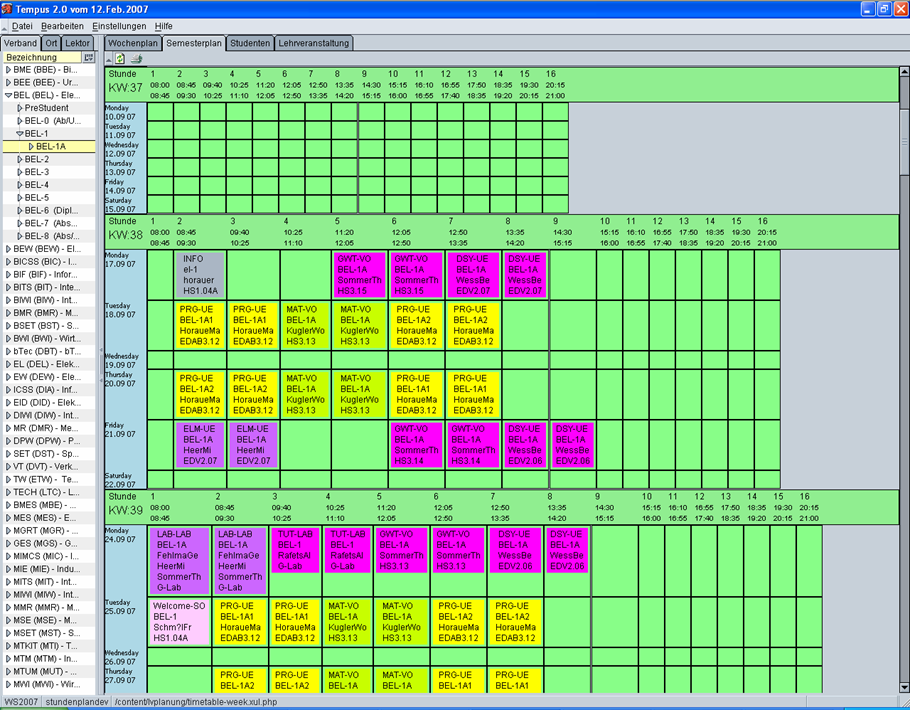
\includegraphics[width=0.8\textwidth]{Tempus_Semesterplan}
	\caption{Karteireiter Semesterplan}
	\label{Semesterplan}
\end {figure}

Wenn Sie im Quellmen� einen anderen Eintrag ausw�hlen, wird der Semesterplan angepasst.
Bei einem Wechsel der Registerkarte bleibt der Semesterplan jedoch unver�ndert erhalten.


\includegraphics{icon_aktualisieren}...Dieser Button aktualisiert den Semesterplan auf den aktuellen Stand.


\includegraphics{icon_drucken}...Ein Klick auf dieses Symbol l�dt den Semesterplan in ein Browser-Fenster von wo aus er gespeichert und gedruckt werden kann.